\section{Zielsetzung}
    \noindent In diesem Versuch wird der Photoeffekt untersucht werden. 
    Dabei soll insbesondere die Energie der ausgelösten Elektronen in Abhängigkeit von der Photonenenergie untersucht werden.\\



\section{Theorie}

    \subsection{Grundlagen}

        \noindent  Die Natur des Lichts lässt sich nicht klar dem Korpuskel- oder dem Wellenmodell zuordnen. 
        In der Quantenelektrodynamik allerdings sind diese beiden Fälle als Grenzfälle enthalten.\\
        Im folgenden Versuch wird bei der Erklärung auf das Korpuskelmodell zurückgegriffen.\\\\

        \noindent Bei diesem Versuch wird eine Metallplatte mit monochromatischem Licht bestrahlt. Dabei werden im besten Fall Elektronen aus der Platte gelöst.
        Um diese Elektronen messen zu können befindet sich gegenüber eine weitere Platte, welche im Bezug zur ersten, ein positives Potential besitzt.\\
        Auf Grund des Potentialunterschieds beschleunigen sich dann die Elektronen von der ersten Platte, genannt Photokathode, zu der anderen Platte, genannt Auffängerkathode.\\
        Dort ensteht dann an abfließender Strom, welcher mit einem Amperemeter gemessen wird.\\

        \noindent Schematisch dargestellt findet man diesen Aufbau in der folgenden Abbildung \ref{img:schem}. 

        \begin{figure}[H]
            \centering
            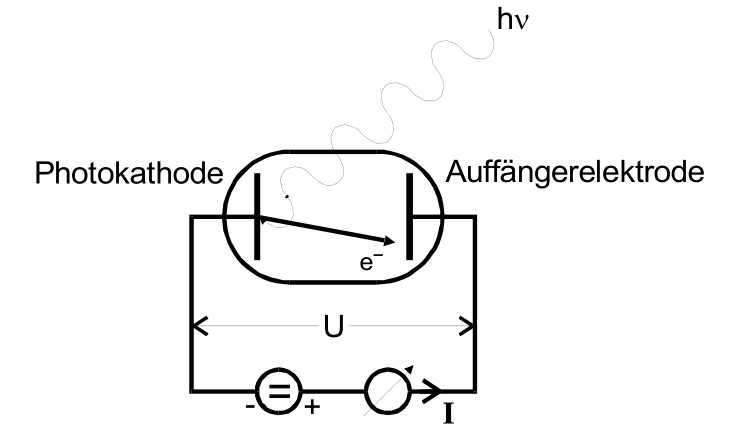
\includegraphics[width=0.65\textwidth]{latex/images/Schaltkreis.PNG}
            \caption{Der schematische Aufbau der zur Untersuchung des Photoeffekts dient.\protect \cite{500}.}
            \label{img:schem}
        \end{figure}

        \noindent Für diesen Versuch gilt, dass die Anzahl der herausgelösten Elektronen proportional zur Intensität des Lichts, 
        die maximale kinetische Energie der Elektronen proportional zur Frequenz des Lichts und die Energie unabhängig von der Intensität ist.\\
        Zusätzlich existiert noch eine Grenzfrequenz des Lichts unterhalb welcher kein Effekt messbar ist.\\
        Dies sind alles Eigenschaften die sich nicht mit dem Wellenmodell nicht erklären lassen. Wenn aber nun angenommen wird, 
        dass sich die gesamte Energie in einem Teilchen mit praktisch verschwindender Ausdehnung konzentriert, lässt sich das ganze erklären.
        Dies sind dann nach dem Korpuskelmodell die sogenannten Photonen.\\
        Sie haben die Energie $\symup{h}\cdot \nu$ wobei $\symup{h}$ das Planck'sche Wirkungsquantum\cite{Planck} ist.\\\\
        \noindent Hier übertragen dann, beim Auftreffen auf die Platte, die Photonen ihre Energie auf die Elektronen.
        




    \subsection{Gegenfeldmethode}